\documentclass{article}
\usepackage{amsmath}
\usepackage{amssymb}
\usepackage{hyperref}
\usepackage{fancyhdr}
\usepackage{graphicx}
\usepackage{setspace}
\usepackage{caption}
\usepackage{wrapfig}
\usepackage{cancel}
\usepackage{pythonhighlight}
\usepackage{float}
\usepackage[a4paper, total={6in, 8in}]{geometry} 
\usepackage{mdframed}
\usepackage{tikz}
\usepackage{mathrsfs}
\usepackage{modalops}


\graphicspath{C:\Users\cmark\OneDrive\Documents\Latex}


\hypersetup{
    colorlinks=true,
    linkcolor=blue,
    urlcolor=cyan,
    citecolor = red
}

\newcommand*\fancypants{\vcenter{\hbox{\includegraphics[width = 2.0em]{fp.png}}}}

\pagestyle{fancy}
\renewcommand{\headrulewidth}{0.4pt}
\renewcommand{\footrulewidth}{0.4pt}
\setlength{\headheight}{18pt}
\setlength{\parindent}{12pt}

\lhead{\large{\bf Carter Garrett}} 
\chead{}
\rhead{\textsc{PHIL 305, Problem Set 9}} 
\lfoot{\today}
\cfoot{}
\rfoot{} 

\newmdtheoremenv{task}{Task}

\usetikzlibrary{arrows,calc,patterns,positioning,shapes}
\usetikzlibrary{decorations.pathmorphing}
\tikzset{
modal/.style={>=stealth',shorten >=1pt,shorten <=1pt,auto,
node distance=1.5cm,semithick},
world/.style={circle,draw,minimum size=1cm,fill=gray!15},
point/.style={circle,draw,fill=black,inner sep=0.5mm},
reflexive/.style={->,in=120,out=60,loop,looseness=#1},
reflexive/.default={5},
reflexive point/.style={->,in=135,out=45,loop,looseness=#1},
reflexive point/.default={25},
}

\begin{document}
    \section{Counterfactuals}
    
        \subsection{}
        \begin{task}
            Demonstrate the following semantic consequences for the material conditional.
        \end{task}

        Note, for this problem let $\mathscr{M}$ be an \textit{SC} model such that $\mathscr{M} = \langle \mathscr{W}, \preceq , \mathscr{I} \rangle$.


            \subsubsection{}
            $$\psi \vDash_{SC} \phi \rightarrow \psi$$

            \textit{Proof.}
            \begin{enumerate}
                \item Assume for reductio that $V_{\mathscr{M}, g}(\phi \rightarrow \psi, w) = 0$ and
                \item $V_{\mathscr{M}, g}(\psi, w) = 1$ for some $w \in \mathscr{W}$.
                \item From (1), we obtain $V_{\mathscr{M}, g}(\phi, w) = 1$ and $V_{\mathscr{M}, g}(\psi, w) = 0$.
                \item We have $V_{\mathscr{M}, g}(\psi, w) = 1$ concurrently with $V_{\mathscr{M}, g}(\psi, w) = 0$. 
                \item $\bot$ (4)
                \item $\therefore \; \psi \vDash_{SC} \phi \rightarrow \psi$
            \end{enumerate}

            \subsubsection{}
            $$\phi \rightarrow \psi \vDash_{SC} \lnot \psi \rightarrow \lnot \phi$$

            \textit{Proof.}
            \begin{enumerate}
                \item Assume for reductio that $V_{\mathscr{M}, g}(\phi \rightarrow \psi , w) = 1$ and
                \item $V_{\mathscr{M}, g}(\lnot \psi \rightarrow \lnot \phi, w) = 0$ for some $w \in \mathscr{W}$.
                \item From (2), we obtain $V_{\mathscr{M}, g}(\lnot \psi , w) = 1$ and 
                \item $V_{\mathscr{M}, g}(\lnot \phi, w) = 0$.
                \item From (3) and (4), we obtain $V_{\mathscr{M}, g}(\psi, w) = 0$ and
                \item $V_{\mathscr{M}, g}(\phi, w) = 1$.
                \item For (1) to obtain, $V_{\mathscr{M}, g}(\phi, w)$ or $V_{\mathscr{M}, g}(\psi, w) = 1$.
                \item But we have obtained (5) and (6), so (7) is not satisfied which means (1) will not hold, or specifically, $V_{\mathscr{M}, g}(\phi \rightarrow \psi, w) = 0$.
                \item $\bot$ (7, 1)
                \item $\therefore \; \phi \rightarrow \psi \vDash_{SC} \lnot \psi \rightarrow \lnot \phi$
            \end{enumerate}

            \subsubsection{}
            $$\phi \rightarrow \psi \vDash_{SC} (\phi \wedge \chi) \rightarrow \psi$$

            \textit{Proof.}
            \begin{enumerate}
                \item Assume for reductio that $V_{\mathscr{M}, g}(\phi \rightarrow \psi, w) = 1$ and
                \item $V_{\mathscr{M}, g}((\phi \wedge \chi) \rightarrow \psi, w) = 0$ for some $w \in \mathscr{W}$.
                \item From (2), $V_{\mathscr{M}, g}(\phi \wedge \chi, w) = 1$ and
                \item $V_{\mathscr{M}, g}(\psi, w) = 0$.
                \item For (3) to obtain, $V_{\mathscr{M}, g}(\phi, w) = 1$ and $V_{\mathscr{M}, g}(\chi, w) = 1$
                \item From (5), if it is the case that $V_{\mathscr{M}, g}(\phi, w) = 1$, then for (1) to obtain, it must be that $V_{\mathscr{M}, g}(\psi, w) = 1$ to satisfy the conditional.
                \item But we have already asserted that $V_{\mathscr{M}, g}(\psi, w) = 0$ in (4).
                \item $\bot$ (7, 6)
                \item $\therefore \; \phi \rightarrow \psi \vDash_{SC}(\phi \wedge \chi) \rightarrow \psi$
            \end{enumerate}

            \subsubsection{}
            $$(\phi \wedge \psi) \rightarrow \chi \vDash_{SC} (\phi \rightarrow (\psi \rightarrow \chi))$$

            \textit{Proof.}
            \begin{enumerate}
                \item Assume for reductio that $V_{\mathscr{M}, g}((\phi \wedge \psi) \rightarrow \chi, w) = 1$ and
                \item $V_{\mathscr{M}, g}(\phi \rightarrow (\psi \rightarrow \chi), w) = 0$ for some $w \in \mathscr{W}$.
                \item (2) implies that $V_{\mathscr{M}, g}(\phi, w) = 1$ and
                \item $V_{\mathscr{M}, g}(\psi \rightarrow \chi, w) = 0$.
                \item (4) implies $V_{\mathscr{M}, g}(\psi , w) = 1$ and 
                \item $V_{\mathscr{M}, g}(\chi, w) = 0$.
                \item If (6), then for (1) to hold, it must be that $V_{\mathscr{M}, g}(\phi \wedge \psi , w) = 0$.
                \item But we have already determined that $V_{\mathscr{M}, g}(\phi, w) = 1$ in (3) and $V_{\mathscr{M}, g}(\psi, w) = 1$ in (5).
                \item $\bot$ (7,8)
                \item $\therefore \; (\phi \wedge \psi) \rightarrow \chi \vDash_{SC} \phi \rightarrow (\psi \rightarrow \chi)$
            \end{enumerate}

        \subsection{}
        \begin{task}
            Demonstrate the following semantic non-consequences for Stalnaker's conditional.
        \end{task}

            \subsubsection{}
            $$\psi \nvDash_{SC} \phi \necif \psi$$

            \textit{Proof.} By countermodel, we can see the non-consequence exemplified. Though $\psi$ obtains for $w$, $\psi$ does not obtain for the maximally close $\phi$ world $v$.

            \begin{center}
                \begin{tikzpicture}[modal]
                    \node[world] (w) [label=below:$v$] {$\phi$};
                    \node[world] (v) [label=below:$@w$,right=of w] {$\psi$};
                    
                    \path[<->] (w) edge (v);
                    %\path[->] (w) edge[reflexive] (w);
                \end{tikzpicture}
            \end{center}

            \subsubsection{}
            $$\phi \necif \psi \nvDash_{SC} \lnot \psi \necif \lnot \phi$$

            \textit{Proof.} By countermodel, we can see that though $\psi$ obtains for the maximally close $\phi$ world $v$, $\lnot \phi$ does not obtain for the maximally close $\lnot \psi$ world $u$.
            \begin{center}
                \begin{tikzpicture}[modal]
                    \node[world] (v) [label=below:$v$] {$\phi$, $\psi$};
                    \node[world] (w) [label=below:$@w$,right=of v] {};
                    \node[world] (u) [label=below: $u$,right=of w] {$\lnot \psi$};
                    
                    \path[<->] (w) edge (v);
                    \path[<->] (w) edge (u);
                    %\path[->] (w) edge[reflexive] (w);
                \end{tikzpicture}
            \end{center}

            \subsubsection{}
            $$\phi \necif \psi \nvDash_{SC} (\phi \wedge \chi) \necif \psi$$

            \textit{Proof.}
            By countermodel, we can see that for $v$, the maximally close $\phi$ world where $\psi$ obtains, we do not necessarily have $\psi$ for the maximally close $\phi, \chi$ world $u$.
            \begin{center}
                \begin{tikzpicture}[modal]
                    \node[world] (w) [label=below:$@w$] {};
                    \node[world] (v) [label=below:$v$,below right=of w] {$\phi$, $\psi$};
                    \node[world] (u) [label=below:$u$,below left=of w] {$\phi, \chi$};
                    
                    
                    \path[<->] (w) edge (v);
                    \path[<->] (w) edge (u);
                    %\path[->] (w) edge[reflexive] (w);
                \end{tikzpicture}
            \end{center}

            \subsubsection{}
            $$(\phi \wedge \psi) \necif \chi \nvDash_{SC} (\phi \necif (\psi \necif \chi))$$

            \textit{Proof.} By countermodel, we demonstrate the semantic non-consequence. 
            It is the case that for the nearest $\phi, \psi$ world $u$ that $\chi$ obtains.
            But it is not the case that for the nearest $\phi$ world $v$, for which the nearest $\psi$ world $t$, that $\chi$ obtains.

            \begin{center}
                \begin{tikzpicture}[modal]
                    \node[world] (w) [label=below:$@w$] {};
                    \node[world] (u) [label=below:$u$,left=of w] {$\phi, \psi, \chi$}; 
                    \node[world] (v) [label=below:$v$,right=of w] {$\phi$};
                    \node[world] (t) [label=below:$t$,right=of v] {$\psi$};

                    \path[<->] (t) edge (v);
                    \path[<->] (w) edge (u);
                    \path[<->] (v) edge (w);

                \end{tikzpicture} 
            \end{center}

        \subsection{}
        \begin{task}
            Do the inferences corresponding to (i) - (iv) above preserve-truth conditions for the 
            English counterfactual conditional? Give an explanation or counterexample in each case.
        \end{task}

        For this section, let $\phi$ represent `it rained.'
        Let $\psi$ represent `we did \textbf{not} climb outside.'
            \subsubsection{}
            $$\psi \vDash_{SC} \phi \necif \psi$$

            \begin{center}
                \textit{``We did not climb, therefore if it rained, we would not have climbed.''}
            \end{center}

            This is not necessarily the case. We might not have climbed for other reasons-- also, we may still have climbed even though it was rainy (e.g. cave climbing). It seems Stalnaker's model and English inference agree:
            $\therefore \psi \nvDash_{SC} \phi \rightarrow \psi$.

            \subsubsection{}
            $$\phi \necif \psi \vDash_{SC} \lnot \psi \necif \lnot \phi$$

            \begin{center}
                \textit{``If it had rained we would not have climbed outside, therefore if we had climbed outside, it would not have rained.''}
            \end{center}

            While seemingly sound, it might not be exactly correct. We can imagine a case where in the nearest $\phi$ world $\psi$ obtains, but in the nearest $\lnot \psi$ world, $\lnot \phi$ does not obtain.
            This is because the maximally similar world changes, and we are capable of a world where we do climb outside ($\lnot \psi$), but it \textit{does} rain ($\phi$).
            Even so, in the English language, by asserting ``if it had rained, we would not have climbed,'' we do not mean to say that anytime we climb outside, it is not raining.
            $\therefore \phi \necif \psi \nvDash_{SC} \lnot \psi \necif \lnot \phi$

            \subsubsection{}
            $$\phi \necif \psi \vDash_{SC} (\phi \wedge \chi) \necif \psi$$

            \begin{center}
                \textit{``If it had rained, we would not have climbed. Therefore, if it had rained, and the rock was dry, we would not have climbed outside.''}
            \end{center}

            I strategically chose $\chi$ to represent `the rock was dry.' We can see how this semantic consequence may not necessarily hold.
            If we have a maximally similar world $u$ where $\phi$ the case along with $\psi$, we can also have another maximally similar $(\phi \wedge \chi)$ world $v$ where $\psi$ does not obtain. 
            In our case, the day may be rainy and the rock may be dry, so we could have climbed outside.
            $\therefore \phi \necif \psi \nvDash_{SC} (\phi \wedge \chi) \necif \psi$.

            \subsubsection{}
            $$(\phi \wedge \psi) \necif \chi \vDash_{SC} \phi \necif (\psi \necif \chi)$$

            For this one, we will slightly change the meaning of $\chi$ for clarity. It will represent `the rock was wet.'
            \begin{center}
                \textit{``If it had rained and we did not climb, the rock would have been wet.
                Therefore, if it had rained, and had we not climbed, the rock would have been wet.''}
            \end{center}

            This one is a bit trickier to navigate. We very well may have a maximally similar $(\phi \wedge \psi)$ world $v$ (where we did not climb and it rained), where $\chi$ (the rock was wet).
            But we may have a separate, maximally similar $\phi$ world $u$, for which another maximally similar $\psi$ world exists where $\chi$ does not obtain.
            In English parlance, just because it may have rained and we did not climb, does not mean the rock was wet. The RHS of the non-consequence can be read as: `If it had rained, and had we not climbed in that instance, the rock would have been wet.' This is not necessarily the case.
            The rock in caves might have been dry, but we did not climb for other reasons. Cave climbing is my favorite anyway.
            $\therefore (\phi \wedge \psi) \necif \chi \nvDash_{SC} \phi \necif (\psi \necif \chi)$.

    \section{Counterfactuals Continued}
    \begin{task}
        Formalize the following argument in the language of \textit{SC} so that its conclusion is an \textit{SC}-semantic consequence of its premises.
        Demonstrate this with an informal semantic argument.
    \end{task}

    \textit{Argument.}
    \begin{enumerate}
        \item Had I flipped the coin, it would have landed either heads or tails.
        \item It is not the case that it would have definitely landed heads if flipped.
        \item So, if I had flipped it, the coin would have landed tails.
    \end{enumerate}

        \subsection{}
        Let $\phi$ represent flipping the coin, and the usual connectives and truth conditions in \textit{SC} apply.
        The first part of the argument can be represented like so:

        \begin{equation}
            \phi \necif (\eta \vee \tau)
        \end{equation}

        Where $\eta$ symbolizes the coin landing heads, and $\tau$ symbolizes the coin landing tails.
        For the second statement, we can symbolize it like so \footnote{Alternatively, we might also write $\lnot \Box (\phi \necif \eta)$ or even $\phi \necif (\lnot \Box \eta)$. The steps in the proof would be similar-- the answer would not vary too greatly.}: 

        \begin{equation}
            \lnot (\phi \necif \Box \eta) 
        \end{equation}
    
        And then the final sentence:

        \begin{equation}
            \phi \necif \tau
        \end{equation}

        We can now put this into an informal semantic argument. 

        \textit{Proof.}
        \begin{enumerate}
            \item Let $V_{\mathscr{M}, g}(\phi \necif (\eta \vee \tau), w) = 1$.
            \item (1) implies that for the maximally similar world $v \in \mathscr{W}$ where $\phi$ obtains, $V_{\mathscr{M}, g}(\eta \vee \tau, v) = 1$.
            \item Now assume that $V_{\mathscr{M},g}(\lnot (\phi \necif \Box \eta), w) = 1$.
            \item (3) means that $V_{\mathscr{M}, g}(\phi \necif \Box \eta, w) = 0$ (by the truth conditions for $\lnot$).
            \item From (4), it must be that $V_{\mathscr{M},g}(\phi, v) = 1$ for every maximally similar $\phi$ world $v \in \mathscr{W}$, and also that
            \item $V_{\mathscr{M},g}(\Box\eta, v) = 0$ for every maximally close $\phi$ world $v\in \mathscr{W}$ (where $v$ is unique in \textit{SC}).
            \item (6) implies that $V_{\mathscr{M},g}(\eta, q) = 0$ for every world $q \in \mathscr{W}$ s.t. $R_{vq}$.
            \item And lastly, (7) means that $V_{\mathscr{M}, g}(\eta, v) = 0$ since $R_{vv}$.
            \item For (1) to hold, it \textit{cannot} be that $V_{\mathscr{M}, g}(\phi, v) = 1$ while $V_{\mathscr{M}, g}(\eta \vee \tau, w) = 0$.
            \item From (8), we have $V_{\mathscr{M}, g}(\eta, v) = 0$, but for the disjunction in (9) to remain true, namely that $V_{\mathscr{M}, g}(\eta \vee \tau, v) = 1$, it must be that $V_{\mathscr{M},g}(\tau, v) = 1$.
            \item $\therefore \; \phi \necif (\eta \vee \tau) \vDash_{SC} \phi \necif \tau$
        \end{enumerate}

        \subsubsection{}
        \begin{task}
            Specify a countermodel to show that it is also not \textit{LC} valid.
        \end{task}

        \textit{Proof.} By an \textit{LC} countermodel, where distance indicates similarity. That is, if world $\phi$ world $u$ is closer to $w$ than $v$, then $u \leq_w v$.
        In this case, we have $LV_{\mathscr{M},g}(\phi \necif (\eta \vee \tau) , w) = 1$. This is true for $v$.
        But the truth conditions for ($\necif$) in \textit{LC} are such that for \textit{for every $\phi$ world} at least as similar as $v$, $(\eta \vee \tau)$ must obtain.
        It is not necessarily the case that $\lnot \eta$ obtains for those worlds, which means that we do not necessarily obtain $\tau$ at $u$.
        \begin{center}
            \begin{tikzpicture}[modal]
                \node[world] (w) [label=below:$@w$] {};
                \node[world] (v) [label=below:$v$,below right=of w, xshift= 10mm, yshift = -15mm] {$\phi$, $(\eta \vee \tau)$};
                \node[world] (u) [label=below:$u$,below left=of w] {$\phi, \eta, (\eta \vee \tau)$};
                
                
                \path[<->] (w) edge (v);
                \path[<->] (w) edge (u);
                %\path[->] (w) edge[reflexive] (w);
            \end{tikzpicture}
        \end{center}
        

    \subsubsection{}
    \begin{task}
        Is the English argument intuitively valid? Briefly explain your answer.
    \end{task}

    The English argument is most definitely invalid. Anyone who considers flipping a coin would grant that it might land heads or tails.
    And while it is not necessary that the coin lands heads, it is not necessary that the coin lands tails either. 
    This ambiguity is somewhat related to contingency as well-- the coin landing heads will either be true or false.
    Although it is the case that it does not necessarily land heads, there may be at least some world where it \textit{does} land on heads.
    In this world, we must grant that the coin does not land on tails. So although it is not necessary that the coin lands heads (i.e. not all worlds land on heads), there are some where it does.
    And in those worlds, the coin does not land tais, making the conclusion false.

\end{document}